%!TEX TS-program = xelatex

\documentclass[xcolor=table, t]{beamer}

\usetheme{Hannover}
\usecolortheme{rose}

%%% Работа с русским языком
\usepackage[english,russian]{babel}   %% загружает пакет многоязыковой вёрстки
\usepackage{fontspec,xltxtra,xunicode}      %% подготавливает загрузку шрифтов Open Type, True Type и др.
%\defaultfontfeatures{Ligatures={TeX},Renderer=Basic}  %% свойства шрифтов по умолчанию
\setmainfont[Ligatures={TeX,Historic},
SmallCapsFont={Brill},
SmallCapsFeatures={Letters=SmallCaps}]{Brill} %% задаёт основной шрифт документа
\setsansfont{Brill}                    %% задаёт шрифт без засечек
\setmonofont[Ligatures=NoCommon]{DejaVu Sans}
%\usepackage{indentfirst}
%%% Дополнительная работа с математикой
\usepackage{amsmath,amsfonts,amssymb,amsthm,mathtools} % AMS
\usepackage{icomma} % "Умная" запятая: $0,2$ --- число, $0, 2$ --- перечисление

%%% Работа с картинками
\usepackage{wrapfig} % Обтекание рисунков текстом
\usepackage{rotating}
\usepackage{fixltx2e}
\usepackage{hhline}
\usepackage{lscape}

%%% Работа с таблицами
\usepackage{array,tabularx,tabulary,booktabs} % Дополнительная работа с таблицами
\usepackage{longtable}  % Длинные таблицы
\usepackage{multirow} % Слияние строк в таблице

\usepackage{multicol} % Несколько колонок
%%% Страница
%\usepackage{fancyhdr} % Колонтитулы
% 	\pagestyle{fancy}
 	%\renewcommand{\headrulewidth}{0pt}  % Толщина линейки, отчеркивающей верхний колонтитул
% 	\lfoot{Нижний левый}
% 	\rfoot{Нижний правый}
% 	\rhead{Верхний правый}
% 	\chead{Верхний в центре}
% 	\lhead{Верхний левый}
%	\cfoot{Нижний в центре} % По умолчанию здесь номер страницы

\usepackage{setspace} % Интерлиньяж
%\onehalfspacing % Интерлиньяж 1.5
%\doublespacing % Интерлиньяж 2
\singlespacing % Интерлиньяж 1

\usepackage{subfig} % подкартинки
\usepackage{lastpage} % Узнать, сколько всего страниц в документе.
\usepackage{soul} % Модификаторы начертания
\usepackage{bbding}
\usepackage{tikz} % Работа с графикой
\usepackage{pgfplots}
\usepackage{pgfplotstable}
\usepackage{verbatim}

\usepackage{attachfile2}
\usepackage{alltt}

%%% Лингвистические пакеты
%\usepackage{savetrees} % пакет, который экономит место
\usepackage{forest} % для рисования деревьев
\usepackage{vowel} % для рисования трапеций гласных
\usepackage{natbib}
\bibpunct[: ]{[}{]}{;}{a}{}{,}
\usepackage[nogroupskip,nopostdot, nonumberlist]{glossaries}
%\usepackage{glossary-mcols} 
%\setglossarystyle{mcolindex}
\usepackage{philex} % пакет для примеров
\newcommand{\mytem}{\item[$\circ$]}
\addto\captionsrussian{
\renewcommand{\refname}{}}

\usetikzlibrary{patterns}

\usepackage{ulem}
\usepackage[absolute,overlay]{textpos}
\usepackage{hyperref}
\hypersetup{ % Гиперссылки
	colorlinks=true, % false: ссылки в рамках; true: цветные ссылки
	linkcolor=black, % внутренние ссылки
	citecolor=black, % на библиографию
	filecolor=black, % на файлы
	urlcolor=blue % на URL
	}
\setbeamercolor{alerted text}{fg=blue}
\setbeamerfont{frametitle}{size=\large}
%\setbeamersize{text margin left=4mm,text margin right=1mm} 
\setlength{\parindent}{0em}
\setbeamertemplate{frametitle}[default][center]
\addtobeamertemplate{frametitle}{\vspace*{-0.1mm}}{\vspace*{-0.3cm}}
%\addtobeamertemplate{frametitle}{\vspace{-0.5\baselineskip}}
\setbeamertemplate{navigation symbols}{
	\usebeamerfont{footline}%
    \usebeamercolor[fg]{footline}%
    %\hspace{1em}%
    {{\tiny презентация доступна: \href{https://goo.gl/41pC4V}{\textbf{https://goo.gl/41pC4V}}}
    \hspace{6.7cm}
    \insertframenumber/\inserttotalframenumber\vspace{0.5mm}}}
% начало
\title[]{Фон.-типология}
\author[]{Г. Мороз}
\date{30 сентября 2019}
\begin{document}
\frame{\titlepage}
\section{термины}
\begin{frame}{Фонетическая или фонологическая типология?}
\medskip
Исследователи по разному смотрят на \textit{типологию}, однако в области фонологии тоже нет единого мнения. Вот список теорий:
\tiny
\begin{itemize}
\mytem Казанская школа
\mytem ЛФШ
\mytem Американский дискриптивизм
\mytem Пражская школа
\mytem МФШ
\mytem Признаковая теория Якобсона, Фанта и Халле
\mytem Генеративная фонология
\mytem Автосегментная фонология
\mytem Метрическая фонология
\mytem Естественная фонология
\mytem Лексическая фонология
\mytem Атомарная фонология
\mytem Теория Элементов
\mytem Геометрия признаков
\mytem Dependency Phonology
\mytem Government Phonology
\mytem Гармоническая фонология
\mytem Теория Оптимальности и ее разновидности
\mytem Вероятностная фонология
\mytem \ldots \hfill {\large Это только слайд закончился, а не список теорий!}
\end{itemize}
\normalsize
\end{frame}
\begin{frame}{Фонетическая или фонологическая типология?}
\begin{itemize}
\mytem В каждой теории граница между фонетикой и фонологией проходит по разному.  Некоторые ученые отрицают фонологию.
\mytem В каждой теории различны единицы описания:
\begin{itemize}
\mytem в МФШ фонемы, в автосегментной фонологии признаки
\mytem в Теории Оптимальности только ограничения, в генеративной фонологии только правила, в когнитивной фонологии, Element Theory и Goverment Phonology  только образцы/прототипы.
\item[\texttt{😼}] Р. О. Якобсона: /pa/ и [tʃik]
\end{itemize}
\end{itemize}
Значит фонетическая типология?
\begin{itemize}
\mytem фонетика в грамматиках обычно факультативна
\mytem отсутствует универсальный алгоритм исследования фонетики
\mytem фонетические исследования достаточно ресурсозатратны 
\end{itemize}
Я буду говорить \textbf{фон.–типология}, по-русски говорят \textit{фонетическая типология}, по-английски: \textit{Phonological Typology}\medskip
\end{frame}

\begin{frame}{Что делает фон.–типология?}
\begin{itemize}
\mytem классификация фон.–единиц
\vspace{-3mm}
\begin{multicols}{2}
\begin{itemize}
\mytem признаки
\mytem сегменты
\mytem слоги
\mytem ударение
\mytem тоны 
\mytem стопы  (\textsc{sg:} стопа)
\mytem фон.–слова, интонация \\
\hfill и т. п. \ldots
\end{itemize}
\end{multicols}
\vspace{-3mm}
\mytem географическая и статистическая дистрибуция фон.–единиц
\mytem ограничения на последовательности фон.–единиц
\mytem классификация, географическая и статистическая дистрибуция чередований фон.–единиц
\mytem универсалии, см. \href{http://typo.uni-konstanz.de/archive/intro/}{Konstanz  Universals  Archive}
\mytem \textbf{\large + все перечисленное внутри языковых систем} \pause
\item[\texttt{😾}] фонология и фонетика жестовых языков\ldots
\end{itemize} \pause
Что же тогда делает фонологическая теория? \citep{hyman06} считает, что фон.–типология и является фонологической теорией.
\end{frame}
\begin{frame}{substance–directed vs. form–directed typology}
В работе \citep{hyman14} предлагается разделять
\begin{itemize}
\mytem \textbf{substance–directed typology}, в рамках которой исследователя интересует распределение какой–то единицы в мире (генеалогическое vs. ареальное vs. типологическое) 
\mytem \textbf{form–directed typology}, в рамках которой исследователя интересует все логические возможности в рамках некой модели:
\begin{itemize}
\mytem какие противопоставления могут быть в фон. системе (Трубецкой)
\mytem как фонологические правила могут взаимодействовать друг с другом (генеративная фонология)
\mytem какие возможны порядки ограничений (теория оптимальности)
\end{itemize}
\end{itemize}
\end{frame}
\section{источники}
\begin{frame}{Источники}
Сегменты и фонологические системы:
\begin{itemize}
\mytem \href{http://www.lapsyd.ddl.ish-lyon.cnrs.fr/lapsyd/index.php}{LAPSyD}
\mytem \href{http://phonetics.ucla.edu/index/sounds.html}{UCLA Phonetics Lab data}
\mytem \href{http://phoible.org/}{PHOIBLE}
\mytem \href{http://eurasianphonology.info/}{The database of Eurasian phonological inventories}
\item[!!!] Peter Ladefoged, Ian Maddieson (1996) The Sounds of the World’s Languages
\end{itemize}
Чередования
\begin{itemize}
\mytem \href{http://reduplication.uni-graz.at/redup/}{база данных редупликаций}
\mytem \href{http://www.diadm.ish-lyon.cnrs.fr/unidia/index.php}{база данных исторических изменений}
\mytem \href{https://agricolamz.github.io/wcad/}{наша база звуковых изменений согласных}
\end{itemize}
Ограничения ОТ
\begin{itemize}
\mytem \href{http://roa.rutgers.edu/}{The Rutgers Optimality Archive}
\end{itemize}
\end{frame}

\section{}
\begin{frame}{Основные функциональные компоненты речепроизводства:} 
\begin{itemize}
\mytem инициация
\mytem фонация
\mytem основная и дополнительная артикуляция
\end{itemize}
\end{frame}
\section{инициация}
\begin{frame}{Инициация}
\vspace{1cm}
 \small
\begin{tabular}{|l|l|l|}
\hline
\multicolumn{1}{|c|}{\multirow{2}[0]{*}{}} & эгрессивная & ингрессивная \\
\multicolumn{1}{|c|}{} & egressive & ingressive \\ \hline
легочная & \multicolumn{1}{c|}{\multirow{2}[0]{*}{большинство звуков}} & \multicolumn{1}{c|}{\multirow{2}[0]{*}{\huge \texttt{\href{http://ingressivespeech.info/}{😽}}}\href{https://www.youtube.com/watch?v=URgdIAz4QNg}{\hspace{2mm} шведское ja}}\\
pulmonic & \multicolumn{1}{c|}{} & 
 \\ \hline
гортанная & \href{http://wals.info/feature/7A}{абруптивные} & \href{http://wals.info/feature/7A}{имплозивные} \\
glottalic & \href{http://wals.info/feature/7A}{ejectives} & \href{http://wals.info/feature/7A}{implosives} \\ \hline
велярное всасывание & \multicolumn{1}{c|}{\cellcolor[HTML]{EFEFEF}} & \href{http://www.youtube.com/watch?v=31zzMb3U0iY}{кликсы, щелкающие} \\
velaric ingressive & \multicolumn{1}{c|}{\cellcolor[HTML]{EFEFEF}} & \href{http://www.youtube.com/watch?v=31zzMb3U0iY}{clicks} \\
\hline
\end{tabular}%
\normalsize
\end{frame}

\section{фонация}
\begin{frame}{Фонация}
\begin{itemize}
\mytem вдох
\mytem шепот
\mytem нейтральная фонация
\mytem придыхательный голос
\mytem \href{https://www.youtube.com/watch?v=YEqVgtLQ7qM}{скрипучий голос}
\end{itemize}
\end{frame}

\section{признаки}
\begin{frame}{Немного истории}
\begin{itemize}
\mytem Казанская школа, Пражский кружок, МФШ:\\
фонема $\approx$ минимальная единица языка, состоящая из набора дифференциальных признаков\\ 
\mytem Генеративная фонология и другие порождающие модели:\\
фонологические правила оперируют дифференциальными признаками (сегменты пишут, просто для удобства):
\end{itemize}
\begin{tabular}{lccccr}
\textsc{sg} & aɾmi\alert{k} & fi\alert{k} & fɾə\alert{ŋ} & muɾ\alert{ɡ} & \citep{buchholz87} \\
\textsc{pl} & aɾmi\alert{c} & fi\alert{c} & fɾə\alert{ɲɟ} & muɾ\alert{ɟ} & албанский  \\
      & ‘враг’ & ‘фига’ & ‘француз’ & ‘монах’ &\\
\end{tabular}
\begin{itemize}
\mytem Автосегментная фонология, Геометрия признаков и др.:
\begin{itemize}
\mytem признаки могут вести себя независимо друг от друга
\mytem не все признаки равноправны 
\mytem признаки организованы иерархически 
\mytem сегменты — результат стечения фонологических признаков \ldots
\end{itemize}
\end{itemize}
\end{frame}

\begin{frame}{Два взгляда на типологию признаков}
\vspace{-2mm}
\begin{itemize}
\mytem устройство признаков универсально: в разных языках представлена лишь часть возможного инвентаря\\(Feature Geometry \citep{clements85} и др.)
\item[\texttt{😒}] т. е. в фонологии всех языков есть признак [$\pm$voice], даже если на поверхностном уровне он не проявляется (пекинский) 
\item[!!!] B. Hayes, K. Zurav и F. van Vugt на основе соответствий IPA и своего универсального набора признаков сделали \href{http://www.linguistics.ucla.edu/people/hayes/120a/Pheatures/Pheatures.jar}{программу}
\vfill
\mytem набор и иерархия признаков зависит от языка\\(Contrastive
Hierarchy, \citep{dresher03} и др.)
\item[\texttt{😒}] если какие–то фонологические признаки отсутстовали в языке, как они тогда могут в нем вдруг появиться или исчезнуть (процесс фонологизации)?
\end{itemize}
\begin{tabular}{cccrr}
I & II &  III && \citep{matisoff73} \\
pá [pā] & pá [pā] & pá [pā] && языки ЮВА\\ 
bá [pa᷇] & bǎ [pa᷄] & pǎ [pa᷄] && звонкие исчезли, тон появился \\ 
\end{tabular}
\end{frame}

\begin{frame}{Носитель признака: палка в колеса}
Согласно работам \citep{cohn93}, \citep{clements03} носителем признака [+nasal] могут быть:\\
\begin{tabular}{llll}
а. & только согласные & /m, n, ŋ/ & корейский (алтайские) \\ 
b. & согласные и гласные & /ĩ, ũ, ã, m, n, ŋ/ & бамана (манде) \\ 
c. & только гласные & /ĩ, ũ, ã/ & иквере (игбоидные) \\ 
d. & на морфеме & /CVC/ⁿ & десано (туканские) \\ 
e. & отсутствует &  & доутаи (папуасские) \\ 
\end{tabular}
\vfill
А что если какие–то сегменты появляются лишь при присоединении слогового признака?
\begin{tabular}{llrr} \hspace{-3mm}
[-phar] & [+phar] &\\ \hspace{-3mm}
\textbf{ʔar}-b-uχ-ib & \textbf{ʡaˤr}-d-aˤq'-un & [Moroz 20??]\\ \hspace{-3mm}
away-\textsc{n}-take.\textsc{pfv-aor} & away-\textsc{f}-go.\textsc{pfv.aor}   &мегебский (н.-даг.) \\ \hspace{-3mm}
‘забрал это’ & ‘она ушла’ & \vspace{2mm} \\ \hspace{-3mm}
\textbf{ħa}-d-irʔ-an & \textbf{ʜaˤ}-d-irʡ-aˤn &\\ \hspace{-3mm}
\textsc{neg-npl-}gather.\textsc{ipfv-hab} &  \textsc{neg-f-}freeze.\textsc{ipfv-hab} &\\ \hspace{-3mm}
‘не собирает их’ & ‘она не замерзает’ &\\ \hspace{-3mm}
\end{tabular} 
\end{frame}
\section{сегменты}
\begin{frame}{Основная и дополнительная артикуляция}
\begin{itemize}
\mytem \vspace{-2mm} место и способ образования
\mytem ряд и подъем
\mytem дополнительная артикуляция
\mytem \href{http://wals.info/feature/1A}{Consonant Inventories}
\mytem \href{http://wals.info/feature/2A}{Vowel Quality Inventories}
\mytem \href{http://wals.info/feature/3A}{Consonant-Vowel Ratio}
\mytem \href{http://wals.info/feature/4A}{Voicing in Plosives and Fricatives}
\mytem \href{http://wals.info/feature/5A}{Voicing and Gaps in Plosive Systems}
\mytem \href{http://wals.info/feature/6A}{Uvular Consonants}
\mytem \href{http://wals.info/feature/7A}{Glottalized Consonants}
\mytem \href{http://wals.info/feature/8A}{Lateral Consonants}
\mytem \href{http://wals.info/feature/9A}{The Velar Nasal}
\mytem \href{http://wals.info/feature/10A}{Vowel Nasalization}
\mytem \href{http://wals.info/feature/10B}{Nasal Vowels in West Africa}
\mytem \href{http://wals.info/feature/11A}{Front Rounded Vowels}
\end{itemize} 
\begin{textblock*}{6cm}(7.5cm, 10mm)
\href{http://www.yorku.ca/earmstro/ipa/}{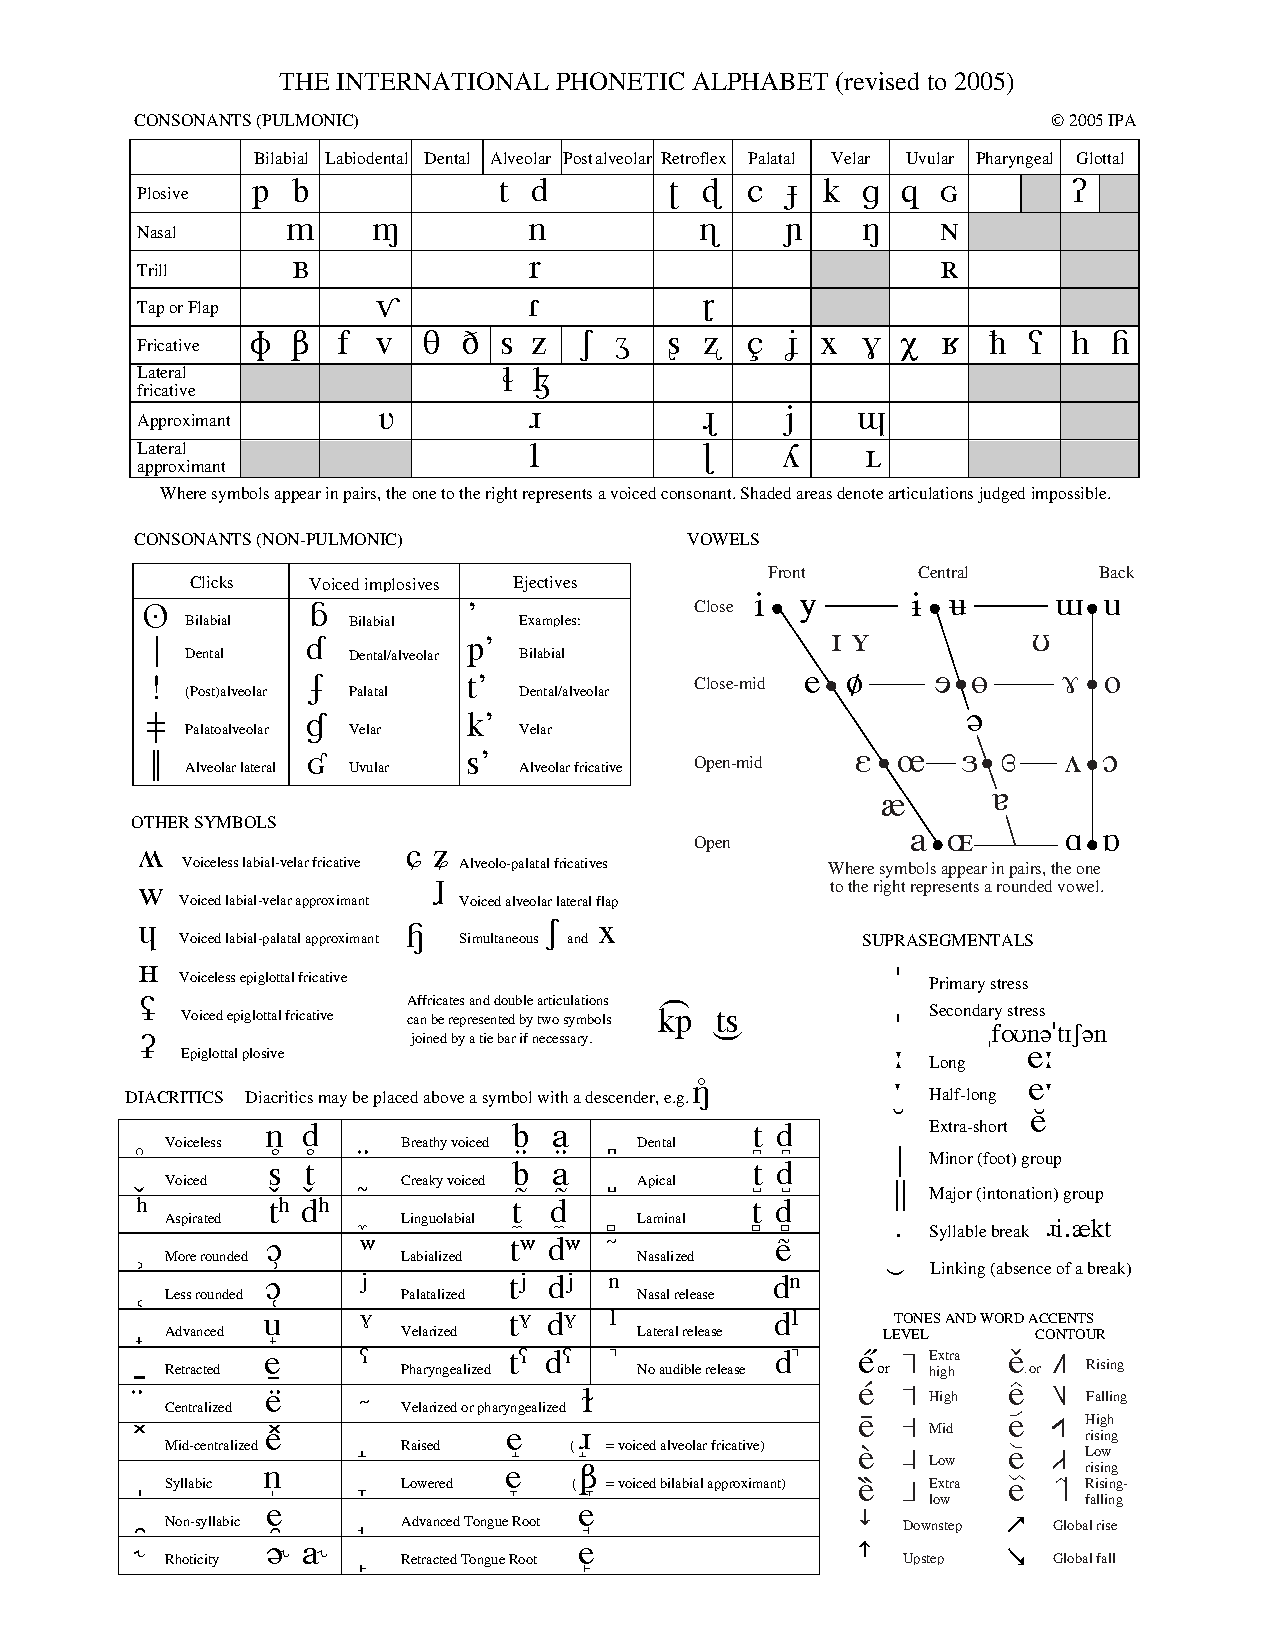
\includegraphics[width=5.7cm]{IPA2005.pdf}}
\end{textblock*}
\end{frame}

\begin{frame}{Размер консонантного инвентаря}
В главе  \href{http://wals.info/feature/1A}{Consonant Inventories \citep{maddieson13cons}} указаны значения данного параметра:\\
\begin{tabular}{ll}
small & 6–14 \\
mod. small & 15–18 \\
average & 22$\pm$3 \\
mod. large & 26–33 \\
large & 34–\ldots \\
\end{tabular}
 \hfill Как получены эти цифры?\\  \pause
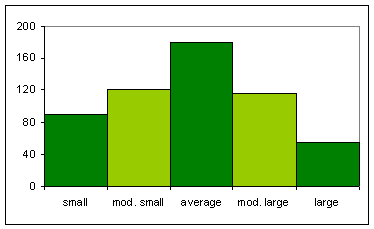
\includegraphics[width=8cm]{conshist.png}
\end{frame}

\begin{frame}{Крайности}
Из работы \citep{hyman08} на основе базы данных UPSID (→ LAPSyD)\\
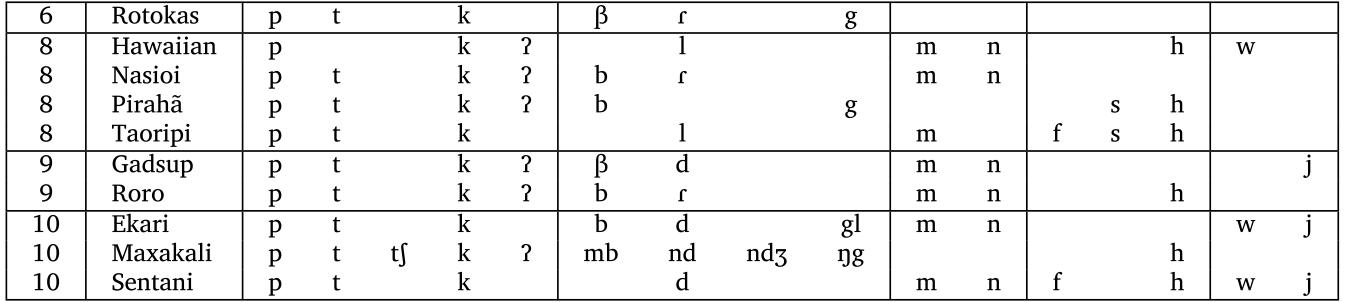
\includegraphics[width=\textwidth]{minimalcons.jpg}\\ 
\begin{itemize}
\mytem везде есть стопы
\mytem везде есть противопоставление по месту
\end{itemize}
\href{http://wals.info/feature/5A}{Voicing and Gaps in Plosive Systems}\\
Больше всего согласных в языке:
\begin{itemize}
\item къхунг — 128 (правда некоторые считают, что 55)
\item убыхский — 85 (за счет абруптивных и фарингализованных)
\item арчинский — 81 (за счет абруптивных и геминат)
\end{itemize}
\end{frame}

\begin{frame}{Как получаются чемпионы?}
На графике представлены две выборки языков из LAPSyD: с абруптивными звуками и без. В среднем, если в языке есть абруптивные, то согласных в нем больше (разница статистически значима: W = 158.5, p-value = 0.0002406 > 0.05, но 27 наблюдений слишком мало).
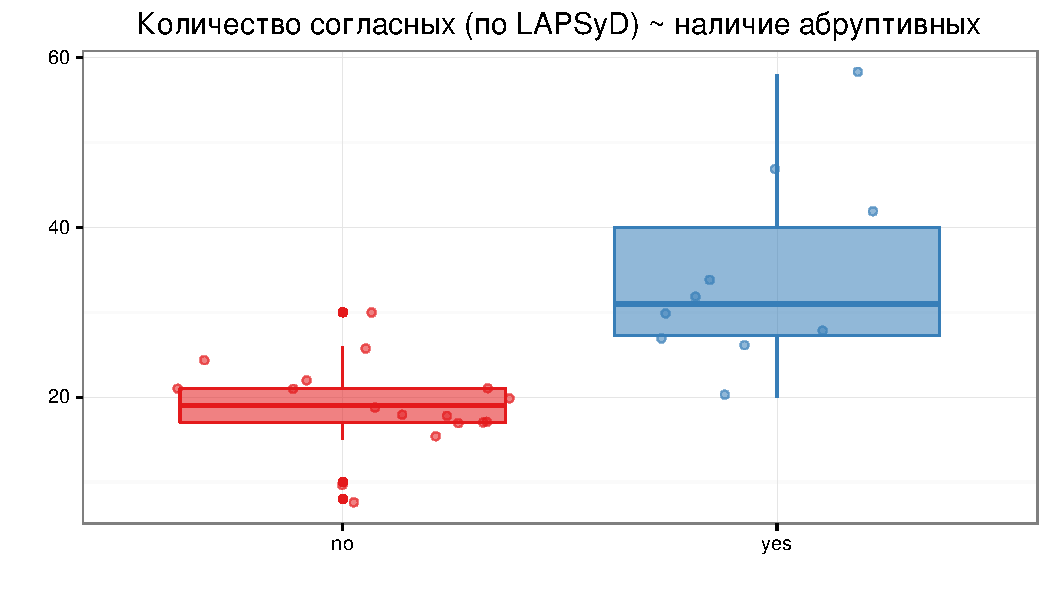
\includegraphics[width=0.90\linewidth]{ejectives.pdf}\\
\vspace{-6mm} Можно посмотреть \href{http://goo.gl/JgrU6g}{\alert{более интерактивный вариант}}.
\end{frame}

\begin{frame}{Гласные}
Еще Трубецкой выделял:
\begin{itemize}
\mytem треугольные системы
\footnotesize
\begin{vowel}[plain]
\putcvowel{i}{1}
\putcvowel{e}{2}
\putcvowel{a}{4}
\putcvowel{u}{8}
\putcvowel{o}{7}
\end{vowel}
\normalsize
\footnotesize
\begin{vowel}[plain]
\putcvowel{i}{1}
\putcvowel{e}{2}
\putcvowel{ɛ}{3}
\putcvowel{a}{4}
\putcvowel{u}{8}
\putcvowel{o}{7}
\putcvowel{ɔ}{6}
\end{vowel}
\normalsize
\mytem четырехугольные системы
\footnotesize
\begin{vowel}[plain]
\putcvowel[l]{i}{1}
\putcvowel[r]{y}{1}
\putcvowel[l]{e}{2}
\putcvowel[r]{œ}{2}
\putcvowel[r]{u}{8}
\putcvowel{a}{4}
\putcvowel[l]{ɯ}{8}
\putcvowel{o}{7}
\end{vowel}
\normalsize
\mytem линейные системы
\footnotesize
\begin{vowel}[plain]
\putcvowel{ə}{11}
\putcvowel{a}{4}
\end{vowel}
\normalsize
\end{itemize}
\end{frame}

\begin{frame}{Крайности}
Из работы \citep{hyman08} по базе данных UPSID\\
\begin{tabular}{|r|r|r|}
\hline
i & u     & a \\
ɪ & ʊ     & a \\
ɪ     & ʊ     & ɐ \\
i     & u     & æ \\
i     & ɯ     & a \\
i     & o     & a \\
ə     & o     & a \\
\hline
\end{tabular}
\small
\begin{vowel}
\putcvowel[l]{iː}{1}
\putcvowel[r]{yː}{1}
\putcvowel[l]{eː}{2}
\putcvowel[r]{øː}{2}
\putcvowel[l]{ɛː ɛ}{3}
\putcvowel[r]{œ}{3}
\putcvowel[l]{aː}{4}
\putcvowel[l]{ʌ}{6}
\putcvowel[r]{ɔ}{6}
\putcvowel[r]{oː}{7}
\putcvowel[r]{uː}{8}
\putcvowel{ə}{11}
\putcvowel{ɪ ʏ}{13}
\putcvowel{ʊ}{14}
\putcvowel{ɐ}{15}
\end{vowel}
\normalsize
\hfill
\small
\begin{vowel}
\putcvowel[l]{i}{1}
\putcvowel[r]{y}{1}
\putcvowel[l]{e}{2}
\putcvowel[r]{ø}{2}
\putcvowel[l]{ɛ}{3}
\putcvowel[r]{œ}{3}
\putcvowel[l]{a}{4}
\putcvowel[r]{ɶ}{4}
\putcvowel[l]{ɑ}{5}
\putcvowel[r]{ɒ}{5}
\putcvowel[l]{ʌ}{6}
\putcvowel[r]{ɔ}{6}
\putcvowel[l]{ɤ}{7}
\putcvowel[r]{o}{7}
\putcvowel[l]{ɯ}{8}
\putcvowel[r]{u}{8}
\putcvowel[l]{ɨ}{9}
\putcvowel[r]{ʉ}{9}
\putcvowel[l]{ɘ}{10}
\putcvowel[r]{ɵ}{10}
\putcvowel{ə}{11}
\putcvowel[l]{ɜ}{12}
\putcvowel[r]{ɞ}{12}
\putcvowel{ɪ ʏ}{13}
\putcvowel{ʊ}{14}
\putcvowel{ɐ}{15}
\putcvowel{æ}{16}
\end{vowel}
\normalsize
\\
\begin{itemize}

\mytem всегда есть противопоставление по подъему
\mytem всегда есть гласный переднего ряда или глайд j
\mytem всегда есть хотя бы один нелабиализованный гласный
\mytem всегда есть хотя бы один гласный заднего ряда
\mytem \href{http://wals.info/feature/2A}{Vowel Quality Inventories}
\end{itemize}
\end{frame}

\begin{frame}{Чем больше … тем…}
Существует миф о том, что чем больше согласных, тем меньше гласных или еще какие-то аналогичные. В работе \citep{maddieson10} получилось так: \medskip\\
\begin{tabular}{|l|l|r|r|r|r|}
\hline
 \multicolumn{2}{|c|}{}  & \multicolumn{4}{c|}{vowels} \\ \cline{3-6}
 \multicolumn{2}{|c|}{}  & \multicolumn{1}{l|}{small} & \multicolumn{1}{l|}{average} & \multicolumn{1}{l|}{large} & \multicolumn{1}{l|}{total} \\ \hline
\multirow{4}[0]{*}{cons} & small & 47 & 153 & 65 & 265 \\ \cline{2-6}
 & average & 34 & 105 & 98 & 237 \\ \cline{2-6}
 & large & 34 & 87 & 57 & 178 \\ \cline{2-6}
 & total & 115 & 345 & 220 & 680 \\ \hline
\end{tabular}
\end{frame}

\section{чередования}
\begin{frame}{Какие бывают звуковые изменения?}
уникальные vs. фонетические vs. морфонологические\\
исторические переход vs. синхронные чередования\\
\vfill
\begin{multicols}{2}
\begin{itemize}
\mytem ассимиляции
\mytem диссимиляции
\mytem гармония
\mytem ослабление
\mytem усиление
\mytem фузия
\mytem расщепление
\mytem элизия
\mytem эпентеза
\mytem чеширизация
\mytem метатеза
\mytem редупликация
\end{itemize}
\end{multicols}
\end{frame}

\begin{frame}{Взаимодействия правил}
С расцветом генеративной фонологии появилась очень известная работа \citep{kiparsky71}, где была введена типология взаимодействия правил.
\begin{itemize}
\mytem питающий порядок (feeding)
\mytem блокирующий порядок (bleeding)
\mytem противопитающий порядок (counterfeeding)
\mytem противоблокирующий порядок (counterbleeding) 
\end{itemize}
\vfill
\begin{tabular}{ccccccccccccc}
\multicolumn{ 5}{c}{feeding} & /EAC/ &  & \multicolumn{ 5}{c}{bleeding} & /XYZ/ \\ 
R1 & A & → & B & /\_C & EBC &  & R1 & Y & → & W & /\_Z & XWZ \\ 
R2 & B & → & D & /E\_ & EDC &  & R2 & X & → & V & /\_Y & — \\ 
\end{tabular}
\bigskip\\ 
\begin{tabular}{ccccccccccccc}
\multicolumn{ 5}{c}{counterfeeding} & /EAC/ &  & \multicolumn{ 5}{c}{counterbleeding} & /XYZ/ \\ 
R1 & A & → & B & /\_C & EBC &  & R1 & Y & → & W & /\_Z & XWZ \\ 
R2 & B & → & D & /E\_ & —  &  & R2 & X & → & V & /\_Y & VWZ \\ 
\end{tabular}
\end{frame}

\begin{frame}{Взаимодействия: питающий порядок}
\textbf{Питающим порядком} (feeding) называют порядок, при котором применение одного правила \textbf{увеличивает} количество контекстов применение другого правила, так что другое правило срабатывает:\\
\vfill
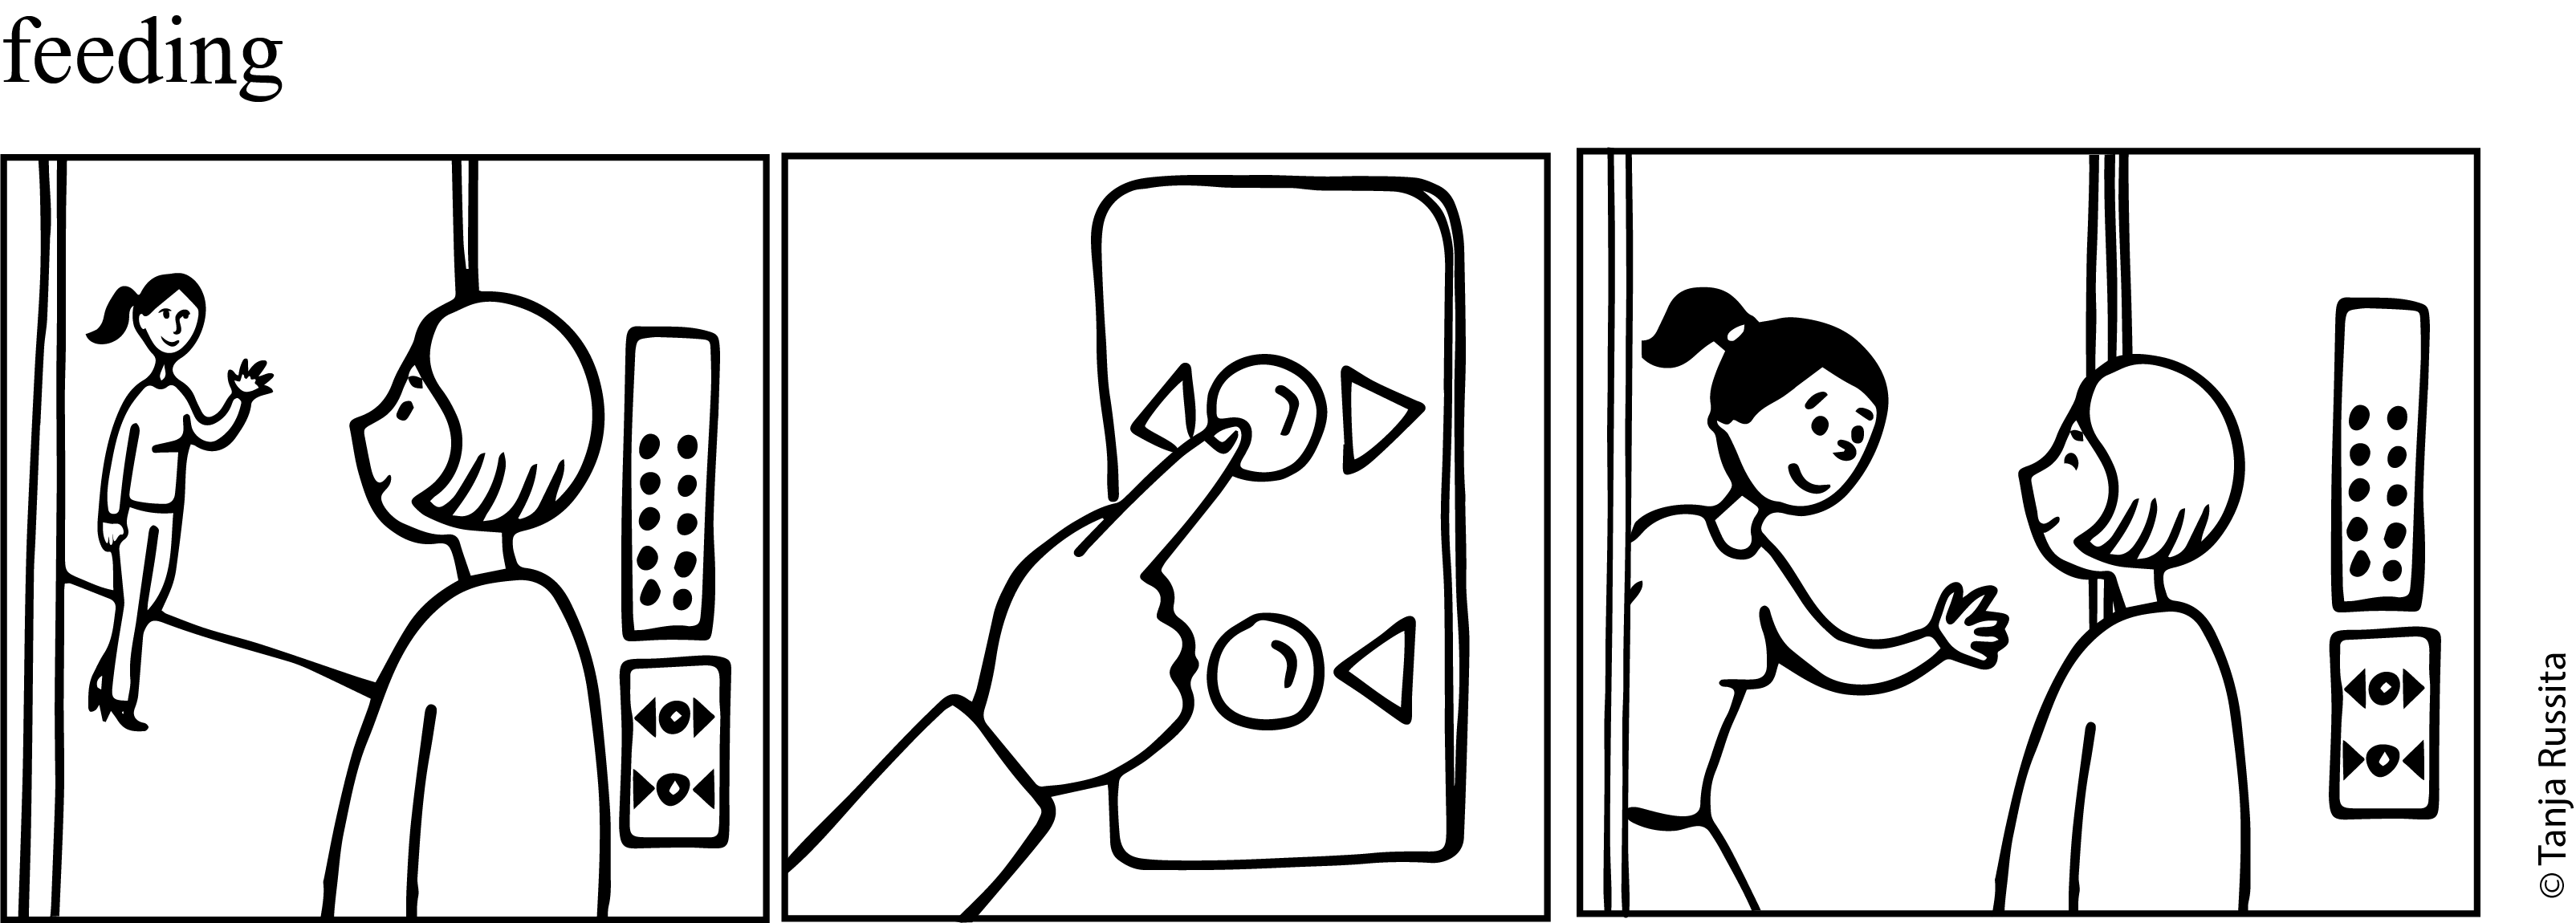
\includegraphics[width=\linewidth]{Russita-feeding.png}
\end{frame}

\begin{frame}{Взаимодействия: питающий порядок}
\textbf{Питающим порядком} (feeding) называют порядок, при котором применение одного правила \textbf{увеличивает} количество контекстов применение другого правила, так что другое правило срабатывает:\medskip\\
\hfill бразильский португальский\\
Палатализация\\
\begin{tabular}{lllllll}
bato & [bá\textbf{t}u] & бить-1\textsc{sg} &  & bate & [bá\textbf{tʃ}i] & бить-3\textsc{sg} \\ 
ardo & [áɾ\textbf{d}u] & жечь-1\textsc{sg} &  & arde & [áɾ\textbf{dʒ}i] & жечь-3\textsc{sg} \\ 
\end{tabular}
\medskip\\
Эпентеза i\\
\begin{tabular}{lll}
pacto & [pák\textbf{i}tu] & соглашение \\ 
captar & [kap\textbf{i}táɾ] & взять в плен \\
psicologia & [p\textbf{i}sikoloʒíɐ] & психология\\
\end{tabular}
\medskip\\ Взаимодействие\\
\begin{tabular}{l|c|c|c|c}
 & /kaptáɾ/ & /áɾdi/ & /advɛ́χsu/ & /futbɔ́w/ \\ \hline
эпентеза i & kap\textbf{i}táɾ & — & ad\textbf{i}vɛ́χsu & fut\textbf{i}bɔ́w \\ \hline
палатализация & — &áɾ\textbf{dʒ}i & a\textbf{dʒ}ivɛ́χsu & fu\textbf{tʃ}ibɔ́w \\ \hline
 & взять в плен  & жжет  & враждебный & футбол \\ 
\end{tabular}
\end{frame}

\begin{frame}{Взаимодействия: блокирующий порядок}
\textbf{Блокирующим порядком} (bleeding) называют порядок, при котором применение одного правила \textbf{уменьшает} количество контекстов применения другого правила, так что другое правило не срабатывает:\\
\vfill
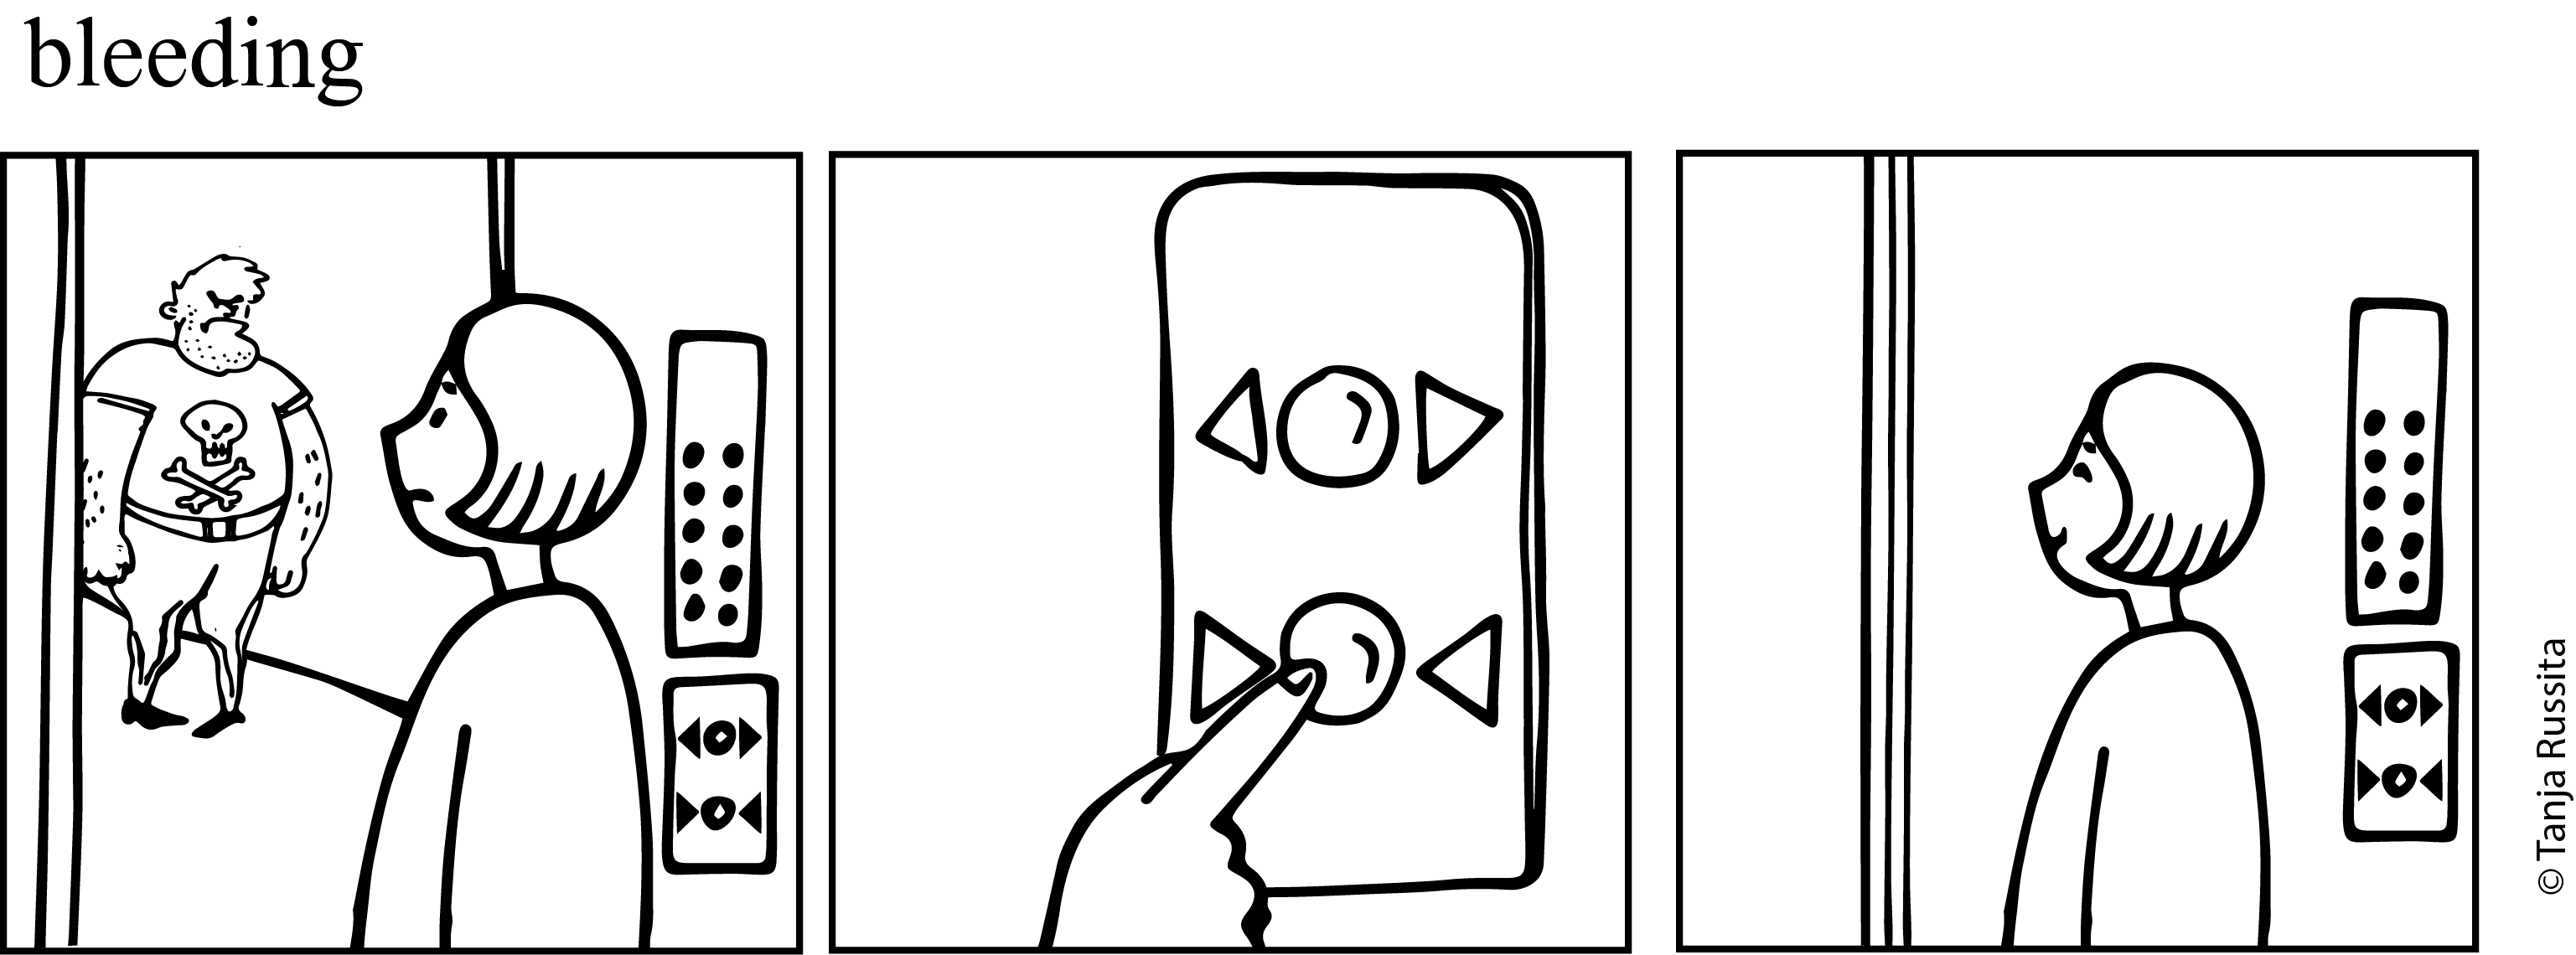
\includegraphics[width=\linewidth]{Russita-bleeding}
\end{frame}

\begin{frame}{Взаимодействия: блокирующий порядок}
\textbf{Блокирующим порядком} (bleeding) называют порядок, при котором применение одного правила \textbf{уменьшает} количество контекстов применения другого правила, так что другое правило не срабатывает:\\
\hfill литовский\\
Эпентеза i\\
\begin{tabular}{lllll}
[at-koːpʲtʲi] & прийти & & [atʲ\textbf{i}-tʲeisʲtʲi] & присудить \\ 

[ap-kalʲbʲetʲi] & оговорить & & [apʲ\textbf{i}-putʲi] & подгнить \\
\end{tabular}
\medskip\\Озвончение\\
\begin{tabular}{lllll}
[at-praʃʲiːtʲi] & спросить  && [a\textbf{d}-gautʲi] & вернуть\\ 

[ap-ʃaukʲtʲi] & объявить  && [a\textbf{b}-gautʲi] &  обмануть  \\
\end{tabular}
\medskip\\Взаимодействие\\
\begin{tabular}{l|c|c|c|c}
 & /ap-putʲi/ &/ap-gautʲi/ & /at-duotʲi/ & /ap-bʲekʲtʲi/ \\ \hline
эпентеза i & apʲi-putʲi & — & atʲi-duotʲi & apʲi-bʲekʲtʲi \\ \hline
озвончение &— & a\textbf{d}-gautʲi & — & — \\ \hline
&подгнить &вернуть & отдать & обежать\\ 
\end{tabular}
\end{frame}

\begin{frame}{Взаимодействия: противопитающий порядок}
\textbf{Противопитающим порядком} (counterfeeding) называют порядок, при котором применение одного правила \textbf{увеличивает} количество контекстов применение другого правила, однако другое правило \textbf{не} срабатывает:\\
\vfill
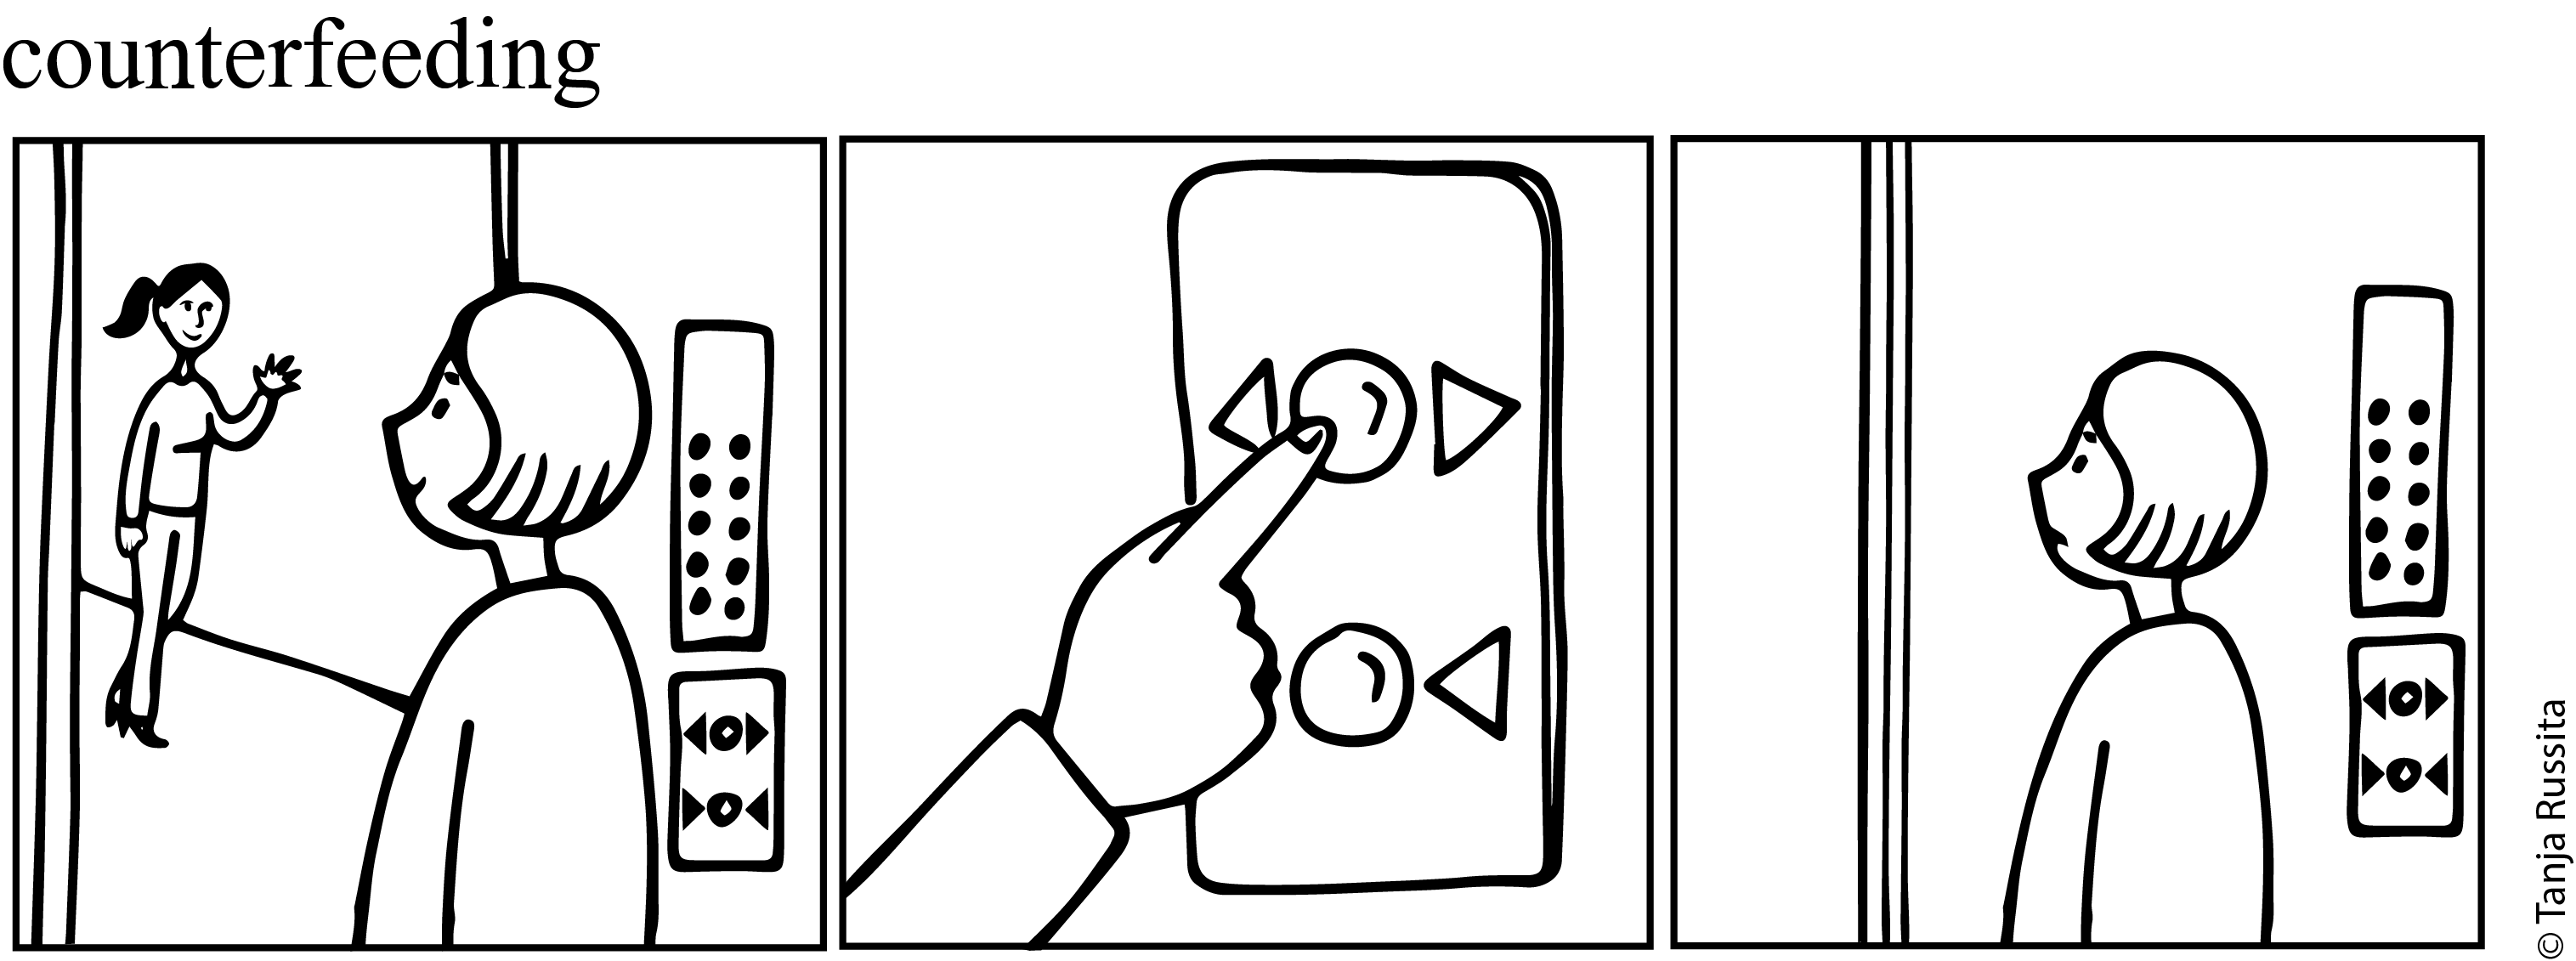
\includegraphics[width=\linewidth]{Russita-counterfeeding.png}
\end{frame}

\begin{frame}{Взаимодействия: противоблокирующий порядок}
\textbf{Противоблокирующим порядком} (counterbleeding) называют порядок, при котором применение одного правила \textbf{уменьшает} количество контекстов применения другого правила, однако другое правило все равно срабатывает:\\
\vfill
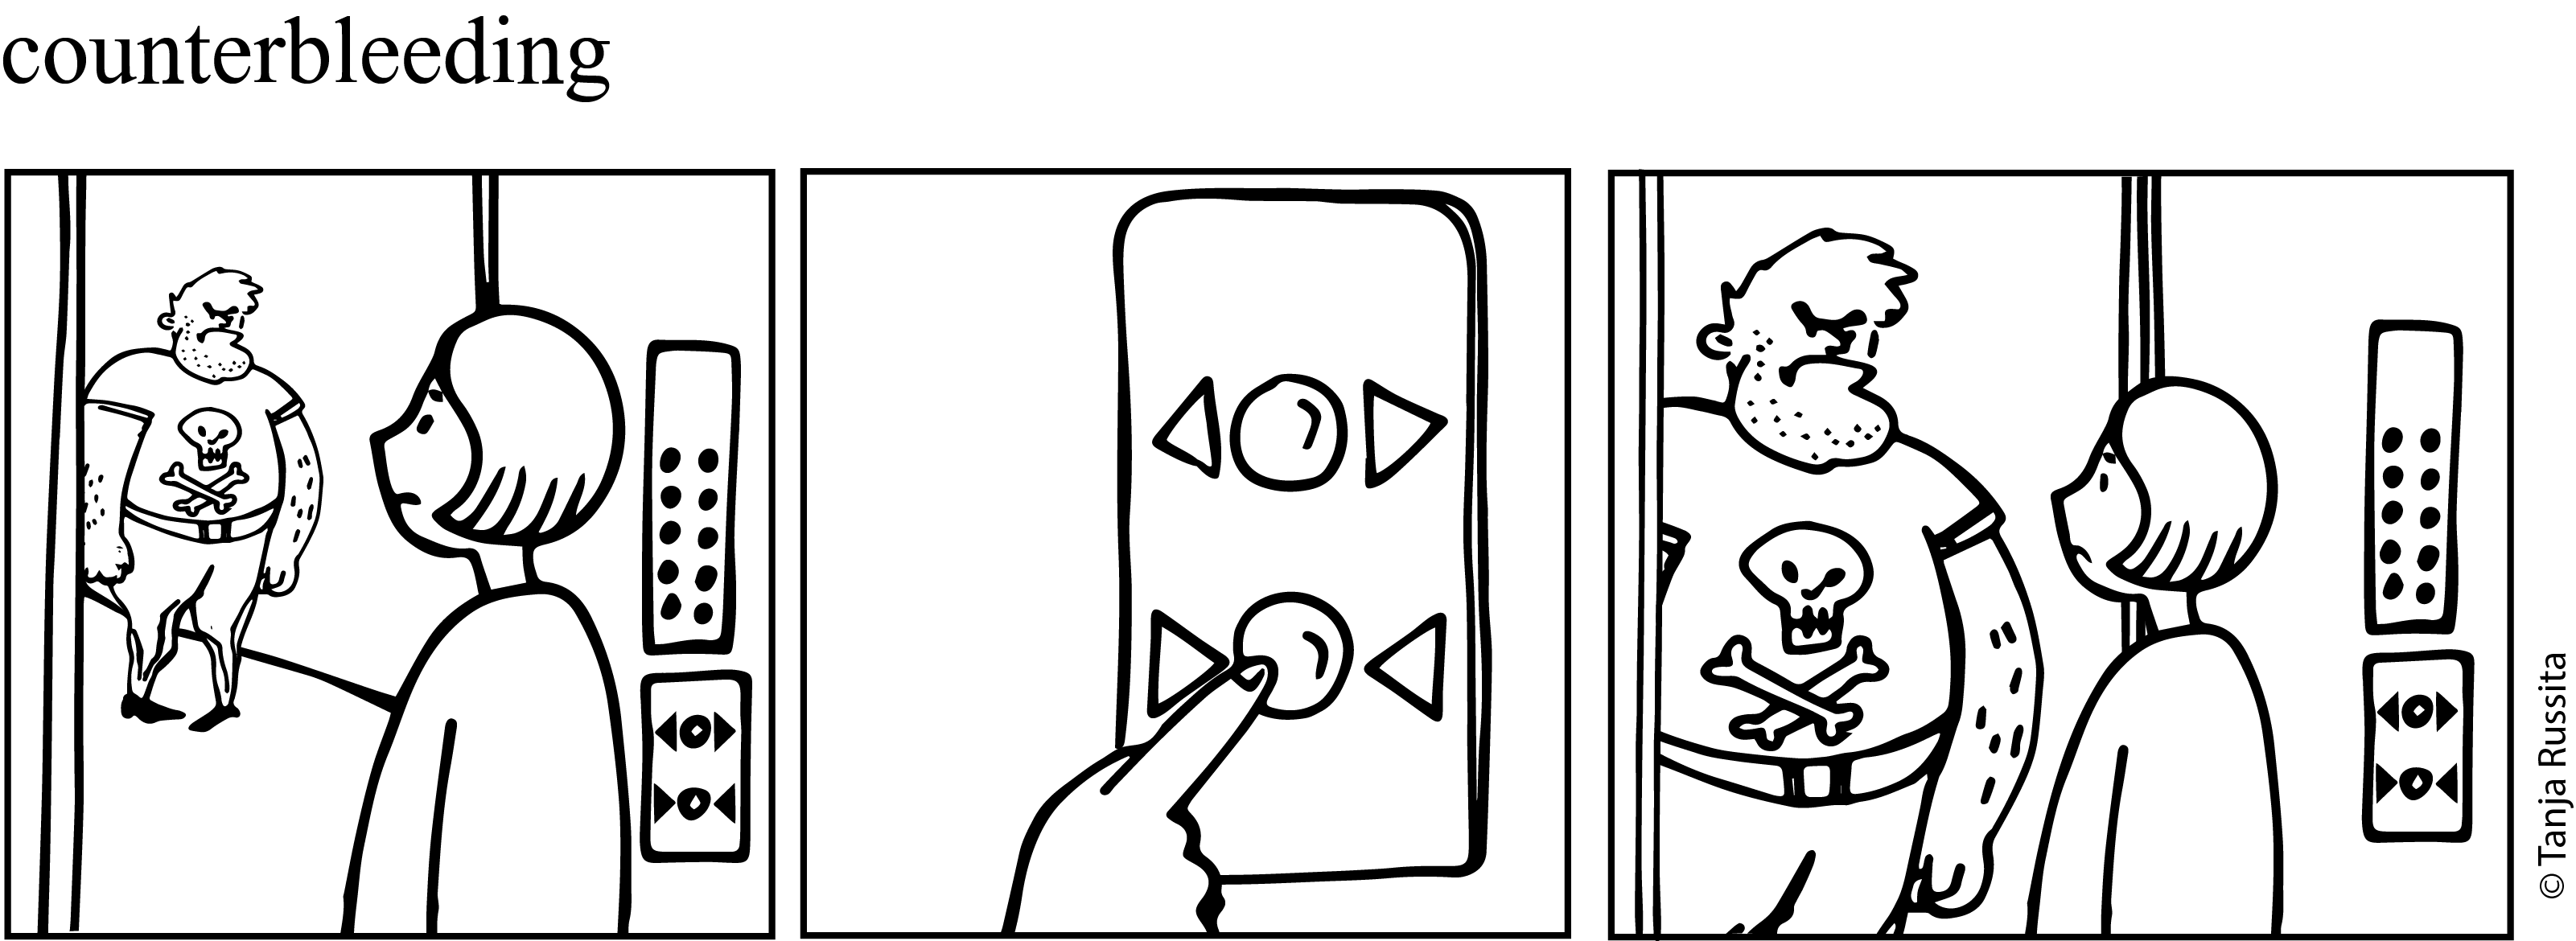
\includegraphics[width=\linewidth]{Russita-counterbleeding.png}
\end{frame}

\section{слоговая структура}
\begin{frame}{Фонотактика}
занимается поиском ограничений на последовательность сегментов внутри фонологических единиц 
\small
\begin{multicols}{2}
\begin{tabular}{ccccc}
C     & C     & V     & L     & C \\
с     & т     & а     & р     & т \\
\end{tabular}
\medskip\\
\begin{forest}
where n children=0{tier=word}{}
[σ [с][т][а][р][т]]
\end{forest}
\medskip\\
\begin{tabular}{cccccccc}
C     & V     & C     & V     & C     & V     & C     & V \\
с     &       & т     & а     & р     &       & т     &  \\
\end{tabular}
\\
\begin{forest}
where n children=0{tier=word}{}
[σ [\textbf{O}nset\\Инициаль, align=center [c][т]][Rhyme[\textbf{N}ucleus\\Ядро, align=center [а]] [\textbf{C}oda\\Финаль, align=center [р][т]]]]
\end{forest}
\end{multicols}
\normalsize

\begin{itemize}
\mytem открытый слог (open/free syllable) — без коды
\mytem закрытый слог (closed/checked syllable) — с кодой
\mytem неприкрытый слог (null onset) — без инициали
\end{itemize}
\href{http://wals.info/feature/12A}{Syllable Structure}: (С)V vs (C)СV(C) vs остальные\medskip
\end{frame}

\begin{frame}{Где проходит слоговая граница?}
Что думают носители? 
\begin{itemize}
\mytem в чем-то сходятся, в чем-то раздрай 
\mytem заики ''справляются'' 
\end{itemize}
Тесты (см. \citep{cote10}): 
\begin{itemize}
\mytem вставка паузы му\ldots ха
\mytem перестановка слогов муха $\rightarrow$ хаму
\mytem редупликация слога муха $\rightarrow$ мумуха
\mytem повторите $n$-ый слог муха $\rightarrow$ му
\mytem замена слога на другой муха $\rightarrow$ ваха
\mytem вставка слога муха $\rightarrow$ муваха
\end{itemize}

А что нам говорят тесты?\\
æpl̩ → æp-æp-pəl, значит æp-pl̩?..\\
Pig Latin : pig → igpay, banana → ananabay\ldots
\end{frame}

\begin{frame}{Амбисиллабические элементы}
\begin{multicols}{2}
\footnotesize
\begin{forest}
where n children=0{tier=word}{}
[ω [σ [O, tier=1[]][R[N, tier=1[æ]] [C, tier=1 [p, name=C2]]]]
[σ [O, tier=1, name=C1][R[N, tier=1[ə]] [C, tier=1 [l]]]]]
\draw [-] (C1.south) -- (C2.north);
\end{forest}
\normalsize

\begin{itemize}
\mytem так часто интерпретируют геминаты: this soup, that~time
\mytem<1->а точно ли всегда есть граница между С и O?..
\mytem также можно смотреть на (пе)ресиллабификацию:
\footnotesize
\begin{forest}
where n children=0{tier=word}{}
[ω [σ [O, tier=1[sˠ]][R[N, tier=1[u]] [C, tier=1 [dˠ, name=C2]]]]
[σ [O, tier=1, name=C1][R[N, tier=1[а]] [C, tier=1 ]]]]
\draw [-] (C1.south) -- (C2.north);
\end{forest}

\normalsize
\mytem может ли ячейку O, N и С занимать признак, а не сегмент?
\end{itemize}
\end{multicols}
\end{frame}

\begin{frame}{Иерархия сонорности}
[Jesperson 1904], \ldots, \citep{clements90} и другие... 
obstruent > nasals > liquids > glides > vowels\\
Не универсалия, но тенденция:\\ 
\begin{itemize}
\mytem английский: twelfths\\ 
\mytem кабардинский: ɕətt't
\mytem \href{http://www.isuma.tv/ourworld/counting-body-parts-nuxalk}{нухалк} (салишские)
\begin{itemize}
\mytem pɬtkn — ‘черёмуха выемчатая’
\mytem q'psttχ — ‘попробуй это!’
\mytem ɬχʷtɬcxʷ — ‘ты насадил на меня’
\mytem χɬp'χʷɬcɬpɬɬs kʷc'  ‘Тогда он владел дёрном канадским’
\end{itemize}
\end{itemize}
\end{frame}

\section{вес слога}
\begin{frame}{Ударение}
\begin{itemize}
\mytem \href{http://wals.info/feature/14A}{фиксированное} 
\mytem подвижное (= лексическое) 
\mytem зависит от веса (база данных StressType)
\begin{itemize}
\mytem LH́\#, H́L\#
\begin{tabular}{c||c|c}
H́H\#     & ĹL\# & 38\\
H́H\#     & LĹ\# & 4\\
HH́\#     & ĹL\# & 8\\
HH́\#     & LĹ\# & 5\\
\end{tabular}

\mytem ударение фиксированное, но есть разница в весе слогов.\\ Моры: L — {μ}, H — {μμ}\\
ударение на третью мору:\\
H́H\# — {μμ́μμ}\#\\
H́L\# — {μ́μμ}\#\\
ĹH\# — { μ́μμ}\#\\
ĹLL\# — { μ́μμ}\#\\
\end{itemize}
\end{itemize}
\end{frame}

\begin{frame}{Что может делать слог тяжелым?}
\begin{itemize}
\mytem кода
\mytem долгие гласные
\mytem гласные полного образования
\mytem высокий тон
\mytem гласный нижнего подъема
\mytem \ldots
\end{itemize}
Подробнее смотрите \citep{gordon06}\\
\footnotesize
\begin{forest}
where n children=0{tier=word}{}
[σ [][{μ}[]]]
\end{forest}
\hspace{4mm}
\begin{forest}
where n children=0{tier=word}{}
[σ [][{μ}[][]]]
\end{forest}
\hspace{4mm}
\begin{forest}
where n children=0{tier=word}{}
[σ [][{μ}[]][{μ}[]]]
\end{forest}
\hspace{4mm}
\begin{forest}
where n children=0{tier=word}{}
[σ [][{μ}, tier=1 [, name=C2]][{μ}, tier=1, name=C1]]
\draw [-] (C1.south) -- (C2.north);
\end{forest}
\normalsize
\end{frame}

\begin{frame}{Компенсаторное удлинение}
Сравните: аттический (сверху) vs лесбосский и фессальский (снизу)
\\\medskip
\small
\begin{forest}
where n children=0{tier=word}{}
[{ω} [σ [{μ}[e]][{μ}[s]]]
[σ [m][{μ}[i]]]]
\end{forest}
$\rightarrow$
\hspace{4mm}
\begin{forest}
where n children=0{tier=word}{}
[{ω} [σ [{μ}, tier=1 [ē, name=C2]][{μ}, tier=1, name=C1]]
[σ [m][{μ}[i]]]]
\draw [-] (C1.south) -- (C2.north);
\end{forest}\\
\begin{forest}
where n children=0{tier=word}{}
[{ω} [σ [{μ}[e]][{μ}[s]]]
[σ [m][{μ}[i]]]]
\end{forest}
$\rightarrow$
\hspace{4mm}
\begin{forest}
where n children=0{tier=word}{}
[{ω} [σ [{μ}, tier=1 [e]][{μ}, tier=1, name=C1]]
[σ [m, name=C2][{μ}[i]]]]
\draw [-] (C1.south) -- (C2.north);
\end{forest}
\normalsize
\end{frame}

\section{}
\begin{frame}
{\huge Спасибо за внимание!\bigskip\\
\normalsize Пишите письма\\
agricolamz@gmail.com
\vspace{-130pt}}
\end{frame}
\begin{frame}[allowframebreaks]{Список литературы}
%\begin{frame}{Список литературы}
\footnotesize
\bibliographystyle{chicago}
\bibliography{/home/agricolamz/work/bibliography.bib}
\end{frame}
\end{document}
